\section{Wavepackets and Fourier Representation}

\subsection{Fourier Inversion Theorem}\label{section_fourier_inversion}

At time $t=0$, any wavefunction $\Psi$ can be written as a superposition of plane waves, as we saw in Section \ref{stationary_phase_approximation}:$$\Psi(x,\,0)=\frac{1}{\sqrt{2\pi}}\int\Phi(k)e^{ikx}\,dk.$$We saw that $\Psi$ is a wavepacket if $\Phi$ is real and localized around some value $k_0$. On the other hand, if we know $\Psi(x,\,0)$, we can calculate $\Phi(k)$ using the \textbf{Fourier inversion theorem}:  

\begin{framedthm}[Fourier inversion theorem]\label{fourier_inversion}
    Given $$\Psi(x,\,0)=\frac{1}{\sqrt{2\pi}}\int\Phi(k)e^{ikx}\,dk,$$ we have $$\Phi(k)=\frac{1}{\sqrt{2\pi}}\int\Psi(x,\,0)e^{-ikx}\,dx.$$
\end{framedthm}

\subsection{Reality Condition}
\label{reality_condition}

We would like to plot $\Psi(x,0)$ as a function of $x$, but for this we need $\Psi$ to be real. Unfortunately, this is not the case. Consider the complex conjugate $$\Psi(x,\,0)^*=\frac{1}{\sqrt{2\pi}}\int\Phi(k)^*e^{-ikx}\,dk.$$We re-parameterize this equation by sending $k$ to $-k$, so that $$\Psi(x,\,0)^*=\frac{1}{\sqrt{2\pi}}\int\Phi(-k)^*e^{ikx}\,dk.$$For $\Psi(x,\,0)$ to be real, we need this to equal $$\Psi(x,\,0)=\frac{1}{\sqrt{2\pi}}\int\Phi(k)e^{ikx}\,dk.$$This is equivalent to the condition $$\int(\Phi(k)-\Phi(-k)^*)e^{ikx}\,dk=0.$$By Theorem \ref{fourier_inversion}, we need $\Phi(k)-\Phi(-k)^*=0$, so $\Phi(-k)^*=\Phi(k)$. Since $\Phi(k)$ is localized at $k_0$, it does not satisfy this condition. Therefore, $\Psi(x,\,0)$ is not real. This forces us to graph $|\Psi(x,0)|$ instead of simply $\Psi(x,0)$.

\subsection{Widths and Uncertainties}\label{widths_uncertainties}
Recall that $\Phi(k)$ is real and localized around $k=k_0$. As shown in Figure \ref{k_uncertainty}, there is then some uncertainty $\Delta k$ in the value of $k$. \footnote{A precise definition of this uncertainty will come later; here, we'll focus on an intuitive understanding of how this uncertainty propagates. }

\begin{figure}[H]
    \centering
    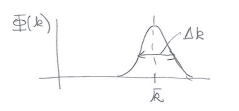
\includegraphics[width=0.5\linewidth]{resources/images/k_uncertainty.png}
    \caption{A graph of $\Phi(k)$ localized around $k=k_0$, with some uncertainty $\Delta k$.}
    \label{k_uncertainty}
\end{figure}

From Section \ref{stationary_phase_approximation}, we know that $|\Psi(x,\,0)|$ peaks when the phase is stationary at $k=k_0$, which occurs at $x=0$. Again, there must be some uncertainty $\Delta x$, as shown in Figure \ref{x_uncertainty}.

\begin{figure}[H]
    \centering
    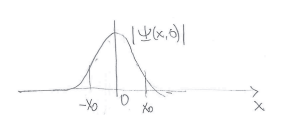
\includegraphics[width=0.5\linewidth]{resources/images/x_uncertainty.png}
    \caption{A graph of $|\Psi(x,0)|$ centered around $x=0$, with some uncertainty $\Delta x=x_0$.}
    \label{x_uncertainty}
\end{figure}

We write $k=k_0+\tilde{k}$. Then we have $$\Psi(x,\,0)=e^{ik_0x}\int\Phi(k_0+\tilde{k})e^{i\tilde{k}x}\,d\tilde{k}.$$Note that the relevant range of integration for $\tilde{k}$ is $[-\frac{\Delta k}{2},\,\frac{\Delta k}{2}]$. For $x=0$, the phase will be stationary for all $\tilde{k}$ and we will get a significant result. On the other hand, for $x\neq 0$, the phase will range over $[-\frac{\Delta k}{2}x,\,\frac{\Delta k}{2}x]$. The total phase excursion is thus $\Delta k\cdot x$. We will get a contribution to the integral as long as this quantity is not too large --- that is, as long as $\Delta k\cdot x\lesssim 1$. Therefore, $\Psi(x,\,0)$ will be sizable in an interval $x\in(-x_0,\,x_0)$ for $\Delta k\cdot x_0\approx 1$. The uncertainty in $x$ is $\Delta x=2x_0$, and since we are approximating, we drop the factor of 2. We therefore have $$\Delta k\,\Delta x\approx1.$$Note that nowhere in this argument did we use quantum mechanics; instead, this is simply a statement about wave packets and Fourier transforms. The physics comes in here: since $p=\hbar k$, we have $\Delta p=\hbar\,\Delta k$. Thus, we have $$\Delta p\,\Delta x\approx \hbar.$$With precise definitions, there is an exact result: $\Delta x\,\Delta p\geq \frac{\hbar}{2}$. This requires more background with uncertainties, which we will cover later. 

\begin{framedexpl}[Square $\Phi(k)$]
    Let $\Phi(k)=\frac{1}{\sqrt{\Delta k}}$ for $-\frac{\Delta k}{2}\leq k\leq\frac{\Delta k}{2}$ and $0$ everywhere else. Then we have $\Phi(k)=-\Phi(k)^*$, so $\Psi(x,\,0)$ is real. In fact,   $$\Psi(x,\,0)=\frac{1}{\sqrt{2\pi}}\int_{-\frac{\Delta k}{2}}^{\frac{\Delta k}{2}}\frac{1}{\sqrt{\Delta k}}e^{ikx}\,dk.$$
    Evaluating, $$\Psi(x,\,0)=\frac{1}{\sqrt{2\pi\Delta k}}\frac{e^{ikx}}{ix}\bigg]^\frac{\Delta k}{2}_{-\frac{\Delta k}{2}}=\sqrt{\frac{\Delta k}{2\pi}}\frac{\sin(\frac{\Delta k\,x}{2})}{(\frac{\Delta k\,x}{2})}.$$We display $\Psi(x,\,0)$ in Figure \ref{square_phi}. We estimate $\Delta x\approx\frac{2\pi}{\Delta k}$, so $\Delta x\,\Delta k\approx 2\pi$.
\end{framedexpl}

\begin{figure}[H]
    \centering        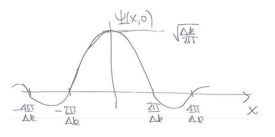
\includegraphics[width=0.5\linewidth]{resources/images/square_phi.png}
    \caption{A graph of $\Psi(x,0)$ for a square $\Phi(k)$.}
    \label{square_phi}
\end{figure}

\section{Time Evolution}
\subsection{Shape Changes in a Wave}\label{shape_changes}

Classical waves maintain a constant shape as they move. However, the Schrödinger equation is first-order in time, so quantum waves also spread outward. We have $$\Psi(x,\,t)=\frac{1}{\sqrt{2\pi}}\int\Phi(k)e^{ikx}e^{-i\omega(k)t}\,dk.$$As in Section \ref{group_velocity}, we expand $\omega(k)$ as $$\omega(k)= \omega(k_0)+ (k-k_0)\frac{d\omega(k)}{dt}\bigg|_{k_0}+\frac{1}{2}(k-k_0)^2\frac{d^2\omega}{dk^2}\bigg|_{k_0}+\ldots$$Recall that $\frac{d\omega}{dk}=\frac{dE}{dp}=\frac{d}{dp}\frac{p^2}{2m}=\frac{p}{m}=\frac{\hbar k}{m}$. Additionally, we have $\frac{d^2\omega}{dk^2}=\frac{\hbar}{m}$ and $\frac{d^3\omega}{dk^3}=0$. Thus, the series actually terminates after the quadratic term! $$\omega(k)= \omega(k_0)+ (k-k_0)\frac{d\omega(k)}{dt}\bigg|_{k_0}+\frac{1}{2}(k-k_0)^2\frac{d^2\omega}{dk^2}\bigg|_{k_0}$$Unlike in Section \ref{group_velocity}, we now consider the quadratic term, so $$e^{-i\omega(k)t}=e^{\ldots -i\frac{1}{2}(k-k_0)^2\frac{\hbar}{m}t}.$$Suppose we start with the wavepacket at $t=0$ and observe as it evolves in time. We have no significant shape change as long as $(k-k_0)^2\frac{\hbar}{m}t\ll 1$. We can estimate $(k-k_0)^2\approx(\Delta k)^2$, since the relevant $k$ terms are within the uncertainty of $\Phi(k)$. Thus, we have $(\Delta k)^2\frac{\hbar t}{m}\ll 1$, which can be rewritten as $$t\ll \frac{m\hbar}{(\Delta p)^2}.$$This is the range of $t$ for which the wave function will not undergo significant shape change. Additionally, we have from Section \ref{widths_uncertainties} that $\Delta x\, \Delta p\approx\hbar$, so we can also write $$t\ll\frac{m}{\hbar}(\Delta x)^2.$$Finally, we can rewrite this as $$\frac{\Delta p}{m}t\ll\Delta x.$$
The packet changes shape because the group velocity $\frac{d\omega}{dk}$ is not constant throughout the packet. The term $\frac{\Delta p}{m}$ represents this uncertainty in the group velocity. There will be appreciable shape change when the uncertainty in velocity, propagating through time, produces position uncertainty comparable to the width $\Delta x$ of the wavepacket. 

\begin{framedquest*}
    For an electron, we have $\Delta x\approx 10^{-10}m$. How long does it remain localized?
\end{framedquest*}

\begin{framedansw*}
    The electron remains localized for time $$t\approx\frac{m}{\hbar}(\Delta x)^2=\frac{mc^2}{\hbar c}\frac{(\Delta x)^2}{c}\approx 10^{-16}s.$$The miniscule time scales for which electrons remain localized provide a technological difficulty for particle accelerators.    
\end{framedansw*}

\subsection{Evolving the Free Particle Wavepacket}
\label{evolving_free_particle}

Suppose you know $\Psi(x,\,0)$ for a free particle and want to find $\Psi(x,\,t)$. This is accomplished in a few steps.

\begin{enumerate}
    \item Calculate $\Phi(k)$ using the Fourier inversion theorem: $\Phi(k)=\frac{1}{\sqrt{2\pi}}\int\Psi(x,\,0)e^{-ikx}\,dx$.
    \item With this, write $\Psi(x,\,0)=\frac{1}{\sqrt{2\pi}}\int \Phi(k)e^{ikx}\,dk$.
    \item To evolve this wavefunction, simply write $$\Psi(x,\,t)=\frac{1}{\sqrt{2\pi}}\int\Phi(k)e^{i(kx-\omega(k)t)}\,dk.$$We have as always that $\hbar\omega(k)=\frac{\hbar^2 k^2}{2m}$. This is a solution to the Schrödinger Equation since it expresses $\Psi(x,\,t)$ as a linear combination of plane waves, each of which is a solution. Since it reduces to $\Psi(x,\,0)$ at $t=0$, it is the unique solution to the Schrödinger Equation that matches the initial conditions.
    \item Perform the integral over $k$, if possible.
\end{enumerate}

\begin{framedexpl}[Evolving the Gaussian]
    Consider the Gaussian wavefunction $$\Psi_a(x,\,0)=\frac{e^{-\frac{x^2}{4a^2}}}{(2\pi)^{1/4}\sqrt{a}}.$$ Since the relevant length scale here is $a$, from Section \ref{shape_changes}, we estimate that the relevant time scale is $\tau\approx\frac{m}{\hbar}a^2$. In fact, it turns out that $\tau=\frac{2ma^2}{\hbar}$. The answer is a bit messy, but we end up with $$|\Psi_a(x,\,t)|^2=\frac{1}{\sqrt{2\pi}}\frac{1}{a(t)}e^{-x^2/2a^2(t)}.$$ Here, $a(t)$ is a time-dependent width given by $a(t)=a\sqrt{1+t^2/\tau^2}$.
\end{framedexpl}

\section{Momentum Space}
\subsection{Delta Functions}\label{delta_functions}

So far, we've been working with wavefunctions that give you the probability of finding a particle at a given position. This is called the \textbf{position space} or \textbf{coordinate space} representation of quantum mechanics. However, we've seen that position and momentum are closely related, and we can reformulate quantum mechanics in terms of \textbf{momentum space}.

Recall from Theorem \ref{fourier_inversion} that $\Psi(x)$ is related to its Fourier transform $\Phi(x)$ by the equations \begin{align*}\Psi(x)&=\frac{1}{\sqrt{2\pi}}\int\Phi(k)e^{ikx}\,dk,\\\Phi(k)&=\frac{1}{\sqrt{2\pi}}\int\Psi(x)e^{-ikx}\,dx.\end{align*}We can think of $\Phi(k)$ as containing the same information as $\Psi(x)$, in that given either one, we can find the other.

Now we have an expression for $\Psi(x)$ in terms of $\Phi(k)$, and vice versa. What if we substitute the expression for $\Phi(k)$ into the first equation? We get \begin{align*}\Psi(x)&=\frac{1}{\sqrt{2\pi}}\int dk\,e^{ikx}\frac{1}{\sqrt{2\pi}}\int\Psi(x')e^{-ikx'}\,dx'\\&=\int dx'\,\Psi(x')\,\underbrace{\frac{1}{2\pi}\int dk\,e^{ik(x-x')}}.\end{align*}Consider the factor indicated by the brace. If $x=x'$, it goes to infinity. However, if $x\neq x'$, it oscillates and prevents the integral from having any contribution. Thus, the factor effectively reduces the $x'$ integral to an evaluation at $x$.\footnote{This is a very hand-wavey argument that probably seems very sketchy --- much of the problem is that the delta function is not really a \textit{function} at all, but a \textit{distribution}, or \textit{generalized function}. All that we need to know about it is that it reduces integrals of other functions to evaluations at points. That being said, if you really need a more rigorous explanation of why this is true, you can check out \href{https://math.stackexchange.com/questions/2340094/why-frac12-pi-int-infty-inftyeiwt-xdw-is-the-dirac-delta-func?noredirect=1&lq=1}{this} Math StackExchange post.} We call it the \textbf{delta function} $$\delta(x-x')=\frac{1}{\sqrt{2\pi}}\int_{-\infty}^{\infty}dk\,e^{ik(x-x')}.$$Note that $\delta(0)=\infty$, and $\delta(ax)=\frac{1}{|a|}\delta(x)$.

\subsection{Parseval's Theorem}\label{section-parseval}

We have found a deep relationship between $\Psi(x)$ and its Fourier transform $\Phi(k)$. We now wish to know how the normalization condition for $\Psi(x)$ (from Section \ref{normalization}) looks in terms of $\Phi(k)$. We have $$\int dx\,\Psi^*(x)\Psi(x)=\int dx\,\frac{1}{\sqrt{2\pi}}\int dk\,\Phi^*(k)e^{-ikx}\,\frac{1}{\sqrt{2\pi}}\int dk'\,\Phi(k')e^{ikx}.$$We have no chance of computing the $k$ and $k'$ integrals, since $\Phi$ is an abstract function. Thus, we rewrite this expression to perform the $x$ integral first: \begin{align*}\int dx\,\Psi^*(x)\Psi(x)&=\int dk\,\Phi^*(k)\int dk'\,\Phi(k')\,\frac{1}{2\pi}\int dx\,e^{i(k'-k)x}\\&=\int dk\,\Phi^*(k)\int dk'\,\Phi(k')\;\delta(k'-k)\\&=\int dk\,\Phi^*(k)\Phi(k).\end{align*}Note that we used the fact that the delta function factor $\delta(k'-k)$ has the effect of evaluating the inner integral at $k$. Our final result is therefore $\int dx\,|\Psi(x)|^2=\int dk\,|\Phi(k)|^2$. This is called \textbf{Parseval's Theorem}:\footnote{In mathematics, a more general version is called Plancherel's theorem.}

\begin{framedthm}[Parseval's Theorem]\label{parseval}
   For a wavefunction $\Psi(x)$ and its Fourier transform $\Phi(k)$, we have $$\int dx\,|\Psi(x)|^2=\int dk\,|\Phi(k)|^2.$$ 
\end{framedthm}

Since we physically associate wavefunctions with momentum eigenstates, we rewrite Parseval's Theorem in terms of $p=\hbar k$. We define $\tilde{\Phi}(p)=\Phi(k)$. We then have \begin{align*}\Psi(x)&=\frac{1}{\sqrt{2\pi}}\int \tilde{\Phi}(p)e^{ipx/\hbar}\frac{dp}{\hbar}\\ \tilde{\Phi}(p)&=\frac{1}{\sqrt{2\pi}}\int\Psi(x)e^{-ipx/\hbar}\,dx\end{align*}For symmetry, we define $\Phi(p)$ so that $\tilde{\Phi}(p)=\Phi(p)\sqrt{\hbar}$. Then these equations become \begin{align*}\Psi(x)&=\frac{1}{\sqrt{2\pi\hbar}}\int {\Phi}(p)e^{ipx/\hbar}dp\\ {\Phi}(p)&=\frac{1}{\sqrt{2\pi\hbar}}\int\Psi(x)e^{-ipx/\hbar}\,dx\end{align*}After a lot of algebra and canceling variables, Theorem \ref{parseval} is unchanged: $$\int dx\,|\Psi(x)|^2=\int dp\,|\Phi(p)|^2.$$

Just as we interpreted $|\Psi(x)|^2\,dx$ in Section \ref{born_rule}, we interpret $|\Phi(p)|^2\,dp$ as the probability to find the particle with momentum in the range $[p,\,p+dp]$. 

\subsection{Fourier Transforms in Three Dimensions}\label{3d-fourier}


In three dimensions, the equations from Theorem \ref{fourier_inversion} take the form \begin{align*}\mathbf{\Psi}(\mathbf{x})&=\frac{1}{(2\pi\hbar)^{3/2}}\int d^3\mathbf{p}\,\mathbf{\Phi}(\mathbf{p})e^{i\mathbf{p}\cdot\mathbf{x}/\hbar},\\ \mathbf{\Phi}(\mathbf{p})&=\frac{1}{(2\pi\hbar)^{3/2}}\int d^3\mathbf{x}\,\mathbf{\Psi}(\mathbf{x})e^{-i\mathbf{p}\cdot\mathbf{x}/\hbar}.\end{align*}Furthermore, there is a delta function in three dimensions, given by $$\delta^3(\mathbf{x}-\mathbf{x}')=\frac{1}{(2\pi)^3}\int d^3\mathbf{k}\,e^{i\mathbf{k}\cdot(\mathbf{x}-\mathbf{x'})}.$$Then we can derive Theorem \ref{parseval} in three dimensions just as in one dimension: $$\int d^3\mathbf{x}\,|\mathbf{\Psi}(\mathbf{x})|^2=\int d^3\mathbf{p}\,|\mathbf{\Phi}(\mathbf{p})|^2.$$